\documentclass[11pt,a4paper]{article}
% Preambulo comun de los reportes de Tecnologias Celulares.
% Cada main.tex hace: \documentclass ... \input{../comun/preambulo.tex}
\usepackage[utf8]{inputenc}
\usepackage[T1]{fontenc}
\usepackage[spanish,mexico]{babel}
\usepackage{graphicx}
\usepackage[margin=2.5cm]{geometry}
\usepackage{amsmath}
\usepackage{amssymb}
\usepackage{booktabs}
\usepackage{tabularx}
\usepackage{array}
\usepackage{float}
\usepackage{setspace}
\usepackage{parskip}
\usepackage{fancyhdr}
\usepackage{textcomp}
\usepackage{xcolor}
\usepackage{caption}
\usepackage{fvextra}
\usepackage[hidelinks]{hyperref}

\onehalfspacing
\setlength{\parskip}{6pt}
\sloppy
\setlength{\emergencystretch}{3em}
\setlength{\headheight}{40pt}
\captionsetup{font=small,labelfont=bf}
\setlength{\tabcolsep}{6pt}

\pagestyle{fancy}
\fancyhf{}
\fancyhead[L]{\includegraphics[width=1cm]{/home/yovick/repos/UAZ-IEI/Assets/UIE.png}}
\fancyhead[R]{\small Tecnologías Celulares}
\fancyfoot[C]{\thepage}
\renewcommand{\headrulewidth}{0.4pt}

\DefineVerbatimEnvironment{codigo}{Verbatim}{%
  breaklines=true,breakanywhere=true,fontsize=\small,frame=single,
  framesep=3pt,rulecolor=\color{gray!50}}

% Figura centrada con pie: \figura[ancho]{archivo}{leyenda}
\newcommand{\figura}[3][0.85]{%
  \begin{center}
    \includegraphics[width=#1\linewidth]{#2}\\[2pt]
    {\small #3}
  \end{center}}

% Portada: \portada{numero}{titulo de la practica}
\newcommand{\portada}[2]{%
\begin{titlepage}
  \thispagestyle{empty}
  \begin{center}
    \vspace*{1cm}
    \includegraphics[width=4.5cm]{/home/yovick/repos/UAZ-IEI/Assets/uaz.png}
    \vspace{0.8cm}

    {\large Universidad Autónoma de Zacatecas}\\[4pt]
    {\large Unidad Académica de Ingeniería Eléctrica}\\[4pt]
    {\normalsize Ingeniería Electrónica Industrial con especialidad en Telecomunicaciones}

    \vspace{1.8cm}
    {\LARGE\bfseries Práctica #1}\\[10pt]
    {\Large\bfseries #2}
  \end{center}

  \vspace{2.2cm}
  \begin{center}
    \begin{tabular}{rl}
      \textbf{Materia:} & Tecnologías Celulares\\
      \textbf{Docente:} & Dr. Víktor Iván Rodríguez Abdalá\\
      \textbf{Alumno:}  & Arnold Yovick Ríos Zaldívar\\
      \textbf{Fecha:}   & Noviembre de 2026\\
    \end{tabular}
  \end{center}
  \vfill
\end{titlepage}}


\graphicspath{{figs/}}

\newcommand{\listado}[1]{%
  \VerbatimInput[fontsize=\scriptsize,breaklines=true,breakanywhere=true,
    frame=single,framesep=2pt,rulecolor=\color{gray!50},numbers=left,
    numbersep=4pt]{#1}}

\begin{document}
\thispagestyle{empty}

% --------------------------------------------------------------- encabezado
\begin{center}
  \includegraphics[width=2.6cm]{/home/yovick/repos/UAZ-IEI/Assets/uaz.png}\\[2mm]
  {\large Universidad Autónoma de Zacatecas}\\
  {\normalsize Unidad Académica de Ingeniería Eléctrica}\\
  {\normalsize Ingeniería Electrónica Industrial con especialidad en Telecomunicaciones}\\[6mm]
  {\LARGE\bfseries Tarea 4}\\[2mm]
  {\large Sistemas de antena múltiple: MIMO, capacidad y códigos espacio-tiempo}\\[5mm]
  {\small
  \begin{tabular}{rl}
    \textbf{Materia:}   & Tecnologías Celulares\\
    \textbf{Docente:}   & Dr. Víktor Iván Rodríguez Abdalá\\
    \textbf{Alumno:}    & Arnold Yovick Ríos Zaldívar\\
    \textbf{Matrícula:} & 35167151 \quad \textbf{Grupo:} VII\\
    \textbf{Fecha:}     & Noviembre de 2026\\
  \end{tabular}}
\end{center}

\vspace{2mm}

Los 15 problemas se resolvieron con \texttt{tarea4.py}. Los canales son
Rayleigh de desvanecimiento lento con entradas $\mathcal{CN}(0,1)$; las
simulaciones Monte Carlo usan detección ML, MMSE e inversa de canal, y el
código de Alamouti con QPSK. Las figuras y los números se regeneran con
\texttt{python3 tarea4.py}.

% ------------------------------------------------------------- problema 1
\section*{Problema 1: matriz de canal}

La función \texttt{canal\_rayleigh(NR,NT,rng)} genera
$H\in\mathbb{C}^{N_R\times N_T}$ con parte real e imaginaria
$\mathcal{N}(0,1/2)$, de modo que $\mathrm{E}|h_{ij}|^2=1$. Para
$(N_R,N_T)=(3,4)$ resultó $\overline{|h_{ij}|^2}=1.10$, consistente con la
varianza unitaria.

% ------------------------------------------------------------- problema 2
\section*{Problema 2: detectores MIMO}

Se repitió la simulación del problema ilustrativo 3 con BPSK y
$H=(\mathcal{N}+j\mathcal{N})/\sqrt{2N_R}$, como en las figuras 3 y 4 del
material. La figura muestra ML, MMSE e ICD para $(2,2)$ y $(2,3)$, con el
combinador de relación máxima (MRC) como referencia.

A 20 dB: en $(2,2)$, ML $9.5\times10^{-5}$, MMSE $2.4\times10^{-3}$ e ICD
$4.5\times10^{-3}$; en $(2,3)$, ML $7.5\times10^{-6}$, MMSE
$8.5\times10^{-5}$ e ICD $1.4\times10^{-4}$. El ML sigue al MRC y alcanza
diversidad $N_R$; los detectores lineales logran $N_R-N_T+1$, tal como en
las figuras 3 y 4.

\begin{figure}[t]
  \centering
  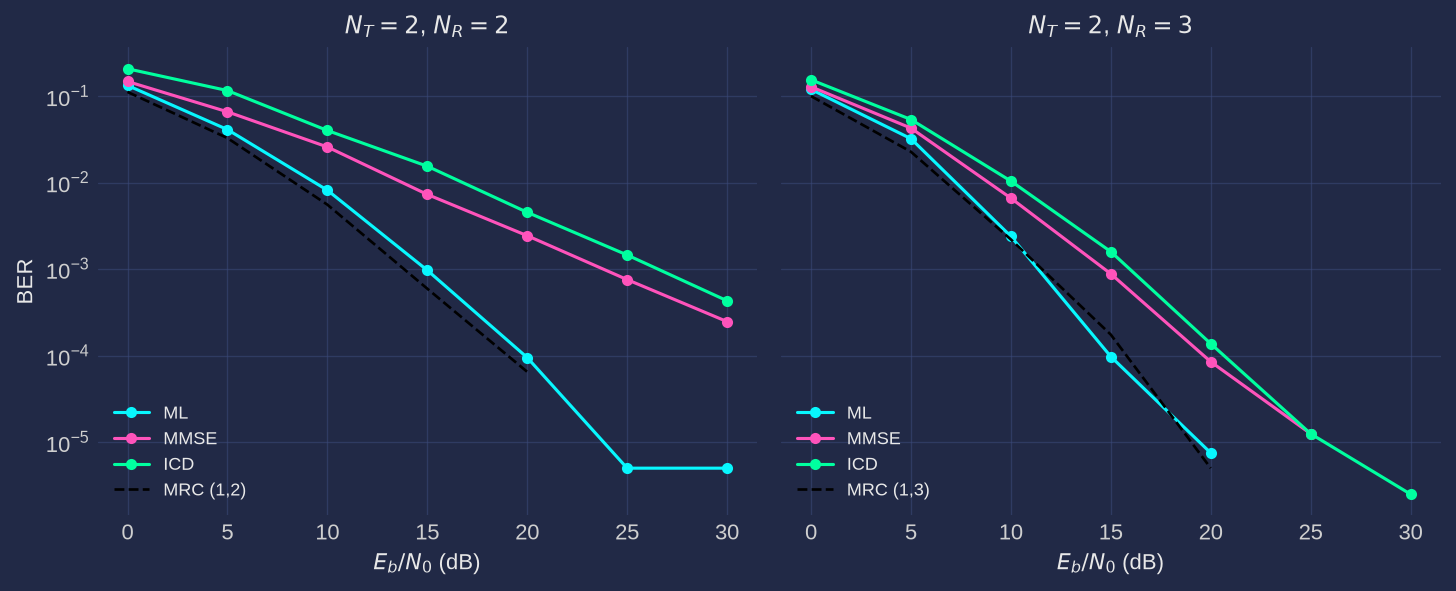
\includegraphics[width=0.9\linewidth]{p2_detectores.png}
  \caption{BER de los detectores ML, MMSE e ICD para $(2,2)$ y $(2,3)$.}
\end{figure}

% ------------------------------------------------------------- problemas 3 y 4
\section*{Problemas 3 y 4: capacidad con matriz fija}

Con $C=\sum_i\log_2(1+\frac{\mathrm{SNR}}{N_T}\lambda_i)$ y
$\lambda_i=\mathrm{eig}(HH^H)$, para el canal $2\times2$ del enunciado
$\lambda=\{1.076,\,4.704\}$ y $C(20\,\text{dB})=13.66$ bps/Hz; para el
$3\times3$, $\lambda=\{1.631,\,2.306,\,7.313\}$ y
$C(20\,\text{dB})=20.01$ bps/Hz.

\begin{figure}[H]
  \centering
  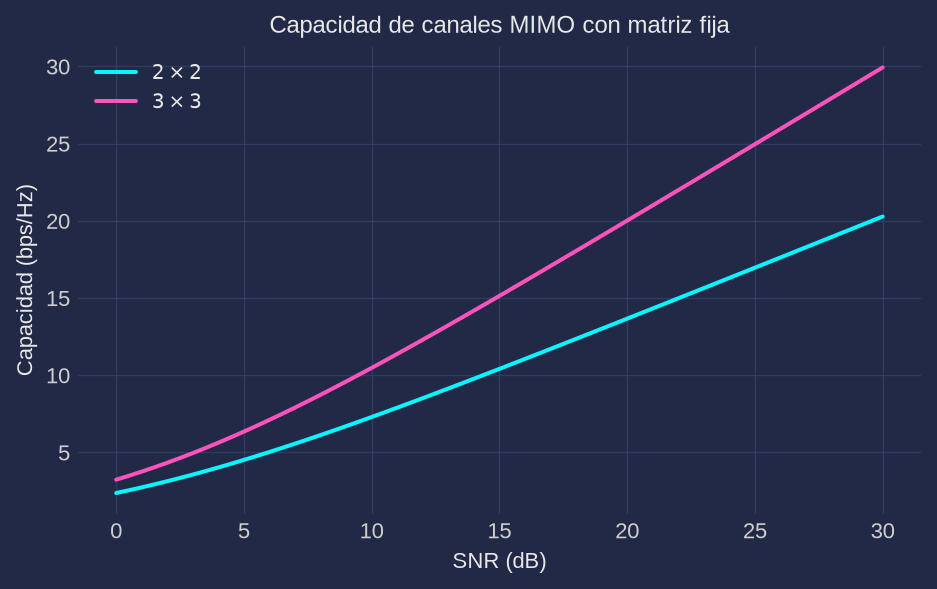
\includegraphics[width=0.72\linewidth]{p34_capacidad_fija.png}
  \caption{Capacidad de los canales $2\times2$ y $3\times3$ con matriz fija.}
\end{figure}

% ---------------------------------------------------------- problemas 5 a 7
\section*{Problemas 5 a 7: capacidad ergódica}

Se promediaron 2000 realizaciones de canal. A 20 dB:

\begin{center}
\begin{tabular}{@{}lcccc@{}}
  \toprule
  & $N=1$ & $N=3$ & $N=5$ & $N=7$ \\
  \midrule
  SIMO ($N_R$) & 5.90 & 7.98 & 8.82 & 9.37 \\
  MISO ($N_T$) & 5.86 & 6.39 & 6.52 & 6.57 \\
  \bottomrule
\end{tabular}
\end{center}

\noindent Para MIMO, $\bar C(20\,\text{dB})=16.68$ bps/Hz con $(3,3)$ y
$27.61$ bps/Hz con $(5,5)$. La capacidad SIMO supera a la MISO porque en
SIMO toda la energía se transmite por una antena, mientras que en MISO se
reparte entre $N_T$.

\begin{figure}[H]
  \centering
  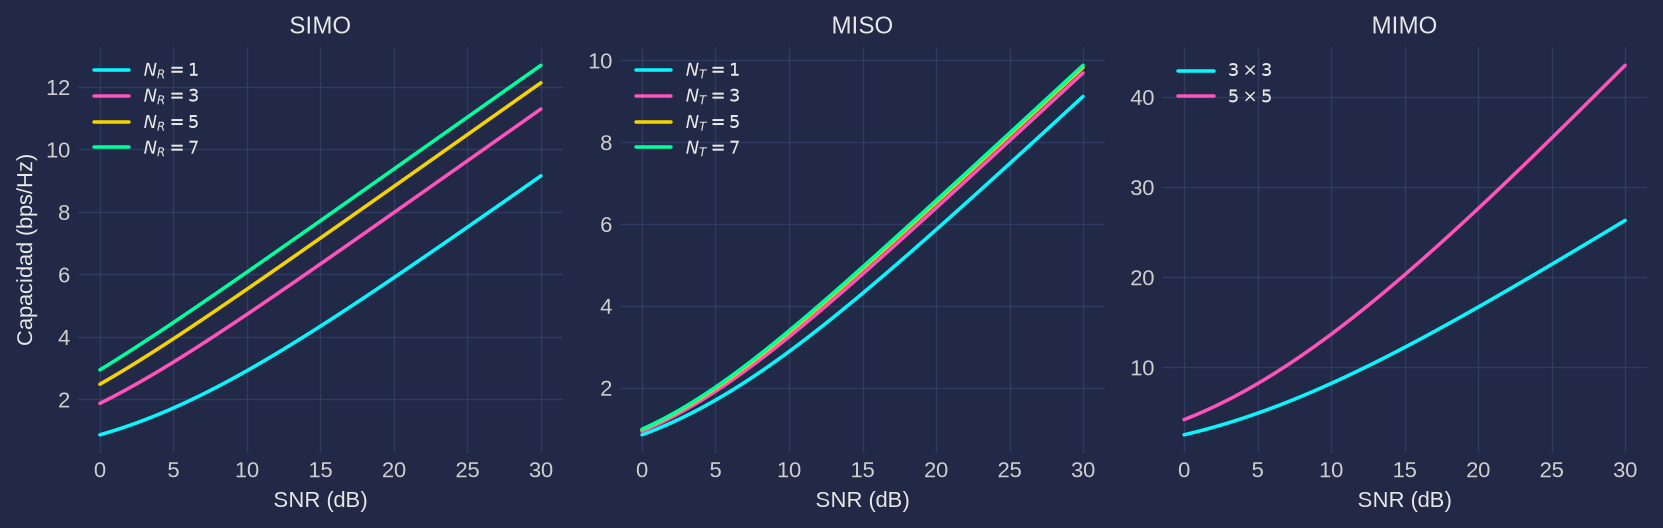
\includegraphics[width=\linewidth]{p567_capacidad.png}
  \caption{Capacidad ergódica de canales SIMO, MISO y MIMO.}
\end{figure}

% ------------------------------------------------------------- problemas 8 y 13
\section*{Problemas 8 y 13: código de Alamouti}

Con QPSK y $E_s=1$, el receptor combina
$\hat s_1=h_1^*y_1+h_2y_2^*$ y $\hat s_2=h_2^*y_1-h_1y_2^*$ y decide por el
punto QPSK más cercano.

Para $2\times1$ la SER a 20 dB es $1.25\times10^{-4}$, con pendiente de
diversidad 2; el SISO sin diversidad queda en $8\times10^{-3}$. Para
$2\times2$ (problema 13, $4\times10^4$ símbolos por punto) la BER es
$1.31\times10^{-4}$ a 10 dB,
$3.1\times10^{-5}$ a 12 dB y $6.25\times10^{-6}$ a 14 dB, con pendiente de
diversidad 4.

\begin{figure}[H]
  \centering
  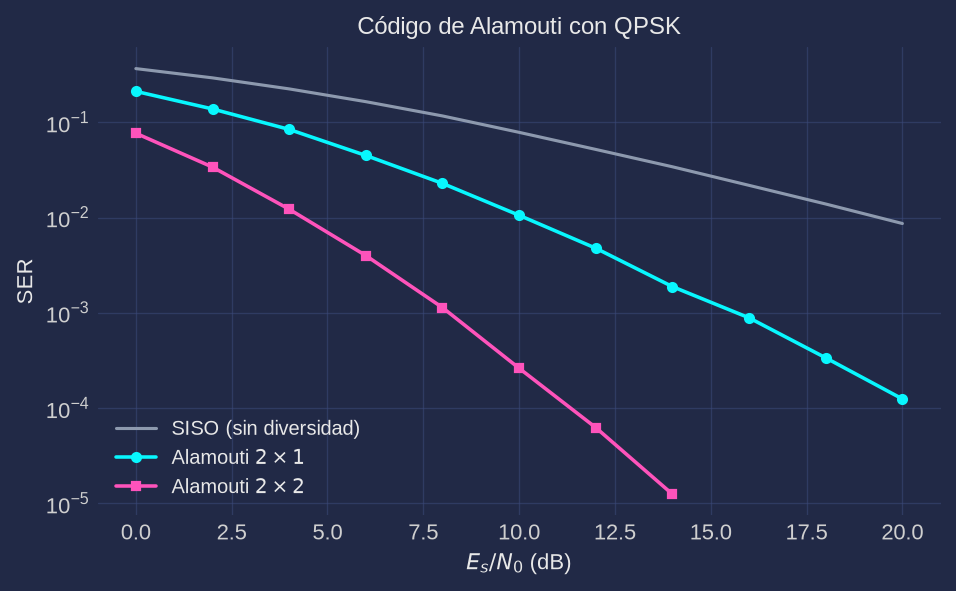
\includegraphics[width=0.72\linewidth]{p8_alamouti.png}
  \caption{SER del código de Alamouti $2\times1$ y $2\times2$ comparada con
  SISO.}
\end{figure}

% ------------------------------------------------------------- problema 9
\section*{Problema 9: ortogonalidad del STBC $4\times1$}

Con $G$ la matriz del enunciado y $c_1,\dots,c_4$ sus columnas,
\begin{equation}
  c_1^Hc_4=(-s_2)s_3+s_3s_2=0,\qquad
  c_1^Hc_1=|s_1|^2+|s_2|^2+|s_3|^2,
\end{equation}
y lo mismo para los demás pares. Por tanto
\begin{equation}
  G^HG=\left(|s_1|^2+|s_2|^2+|s_3|^2\right)I_4 ,
\end{equation}
que se verificó numéricamente con error $8.9\times10^{-16}$. La tasa es
$R_s=3/4$ y, al ser ortogonal con $N_T=4$, el código alcanza diversidad de
cuarto orden.

% ------------------------------------------------------------- problema 10
\section*{Problema 10: detector del STBC $4\times1$}

Las salidas de los correladores en las cuatro ranuras son
\begin{align}
  y_1&=h_{11}s_1+h_{12}s_2+h_{13}s_3+\eta_1,\\
  y_2&=-h_{11}s_2^*+h_{12}s_1^*+h_{14}s_3+\eta_2,\\
  y_3&=h_{11}s_3^*-h_{13}s_1^*+h_{14}s_2+\eta_3,\\
  y_4&=-h_{14}s_1+h_{12}s_3^*-h_{13}s_2^*+\eta_4.
\end{align}
El detector de máxima verosimilitud elige, entre las $4^3=64$ tripletas
4-PSK,
\begin{equation}
  \hat{\mathbf s}=\arg\min_{\mathbf s}\left\|\mathbf y-G(\mathbf s)\mathbf h\right\|^2,
\end{equation}
donde $\mathbf h=[h_{11},h_{12},h_{13},h_{14}]^T$. La prueba numérica
recuperó los 500 símbolos de prueba sin errores. La ortogonalidad de $G$
garantiza la diversidad de orden 4.

% ------------------------------------------------------------- problema 11
\section*{Problema 11: ortogonalidad del STBC de tasa $3/4$}

Con
$H_{31}=\begin{bmatrix}h_{11}&h_{12}&h_{13}\\h_{12}^*&-h_{11}^*&0\\-h_{13}^*&0&h_{11}^*\\0&-h_{13}^*&h_{12}^*\end{bmatrix}$,
cada columna tiene norma $|h_{11}|^2+|h_{12}|^2+|h_{13}|^2$ y los productos
cruzados se cancelan, por ejemplo
\begin{equation}
  c_1^Hc_2=h_{11}^*h_{12}-h_{12}h_{11}^*=0.
\end{equation}
Así,
\begin{equation}
  H_{31}^HH_{31}=\left(|h_{11}|^2+|h_{12}|^2+|h_{13}|^2\right)I_3
\end{equation}
(error numérico $4.4\times10^{-16}$), de modo que
$\hat{\mathbf s}=H_{31}^H\mathbf y/\|h\|^2$ y el sistema alcanza diversidad
de tercer orden.

% ------------------------------------------------------------- problema 12
\section*{Problema 12: matriz de canal para $(4,2)$}

La matriz se genera con la misma función del problema 1:
\texttt{H = canal\_rayleigh(2, 4, rng)}, es decir, una matriz $2\times4$ de
entradas $\mathcal{CN}(0,1)$, independientes entre ranuras y antenas.

% ------------------------------------------------------------- problema 14
\section*{Problema 14: diversidad del Alamouti $2\times2$}

Para dos antenas receptoras se apilan las dos ecuaciones de Alamouti y
queda una matriz equivalente $4\times2$ con
\begin{equation}
  H_{\text{eq}}^HH_{\text{eq}}
  =\left(|h_{11}|^2+|h_{12}|^2+|h_{21}|^2+|h_{22}|^2\right)I_2
\end{equation}
(error numérico $1.8\times10^{-17}$). Los cuatro coeficientes son
Gaussianos independientes, así que la señal útil se suma coherentemente
mientras el ruido lo hace de forma incoherente: la diversidad es de cuarto
orden.

% ------------------------------------------------------------- problema 15
\section*{Problema 15: código de trellis de 8 estados}

La tabla resume el codificador de la figura 1: para cada estado y símbolo
de entrada (0 a 3) se indica el estado siguiente y el par de símbolos
4-PSK transmitidos por las dos antenas.

\begin{center}
\small
\begin{tabular}{@{}c|ccc|ccc|ccc|ccc@{}}
  \toprule
  Estado & \multicolumn{3}{c|}{entrada 0} & \multicolumn{3}{c|}{entrada 1}
  & \multicolumn{3}{c|}{entrada 2} & \multicolumn{3}{c}{entrada 3}\\
  & sig. & $s_1$ & $s_2$ & sig. & $s_1$ & $s_2$ & sig. & $s_1$ & $s_2$
  & sig. & $s_1$ & $s_2$\\
  \midrule
  0 & 0 & 0 & 0 & 1 & 1 & 1 & 2 & 2 & 2 & 3 & 3 & 3\\
  1 & 1 & 1 & 1 & 2 & 2 & 2 & 3 & 3 & 3 & 4 & 2 & 0\\
  2 & 2 & 2 & 2 & 3 & 3 & 3 & 4 & 2 & 0 & 5 & 3 & 1\\
  3 & 3 & 3 & 3 & 4 & 2 & 0 & 5 & 3 & 1 & 6 & 0 & 2\\
  4 & 4 & 2 & 0 & 5 & 3 & 1 & 6 & 0 & 2 & 7 & 1 & 3\\
  5 & 5 & 3 & 1 & 6 & 0 & 2 & 7 & 1 & 3 & 0 & 0 & 0\\
  6 & 6 & 0 & 2 & 7 & 1 & 3 & 0 & 0 & 0 & 1 & 1 & 1\\
  7 & 7 & 1 & 3 & 0 & 0 & 0 & 1 & 1 & 1 & 2 & 2 & 2\\
  \bottomrule
\end{tabular}
\end{center}

\noindent Para la entrada $(3,2,2,3,0,1,0,0,1,2)$ el codificador transmite
$s_1=(3,3,1,2,2,3,3,3,2,0)$ y $s_2=(3,0,0,3,0,1,0,0,3,0)$.

% ------------------------------------------------------------- conclusiones
\section*{Conclusiones}

\begin{itemize}
  \item El ML explota la diversidad $N_R$ y sigue al MRC; MMSE e ICD pierden
        diversidad ($N_R-N_T+1$).
  \item La capacidad MIMO crece linealmente con el número de pares de
        antenas; SIMO supera a MISO para la misma norma de canal.
  \item Alamouti da diversidad 2 con $2\times1$ y 4 con $2\times2$; las
        pendientes simuladas coinciden con esos órdenes.
  \item Los códigos $G$ y $H_{31}$ son ortogonales, lo que desacopla los
        símbolos y garantiza diversidad 4 y 3, respectivamente.
  \item El codificador de trellis de 8 estados se implementó con una tabla
        de transición y salidas 4-PSK.
\end{itemize}

% ------------------------------------------------------------------ codigo
\appendix
\section{Código}
\listado{tarea4.py}

\end{document}
